\chapter{Order From Understanding Disorder}

This chapter follows J. Krishnamurti's San Diego conversation with Allan W. Anderson on order, disorder, thought, measurement, comparison, and observation. The source material is credited to J. Krishnamurti and the Krishnamurti Foundation Trust, with curation by LazyingArt LLC through Video2Book. No validated blackboard equation or diagram frames remain for this lecture, so the notation below is intentionally modest. It is not a substitute for the spoken inquiry; it is a compact way of keeping its structure visible.

The movement of the conversation is simple to state and difficult to follow through: we begin with the world's disorder, discover that imposed order belongs to that disorder, and then ask whether order can come from understanding disorder without an observer who tries to control it.

\section{The Question Of Order In Freedom}

Anderson opens by proposing that they discuss order. Krishnamurti immediately places the word inside the previous field of inquiry: freedom, responsibility, and relationship. That placement matters. We are not asking first about social neatness, discipline, or obedience. We are asking what order means when freedom has not already been sacrificed.

A useful caution is

\begin{equation}
\text{order in freedom} \neq \text{order by control}.
\end{equation}

The conversation then refuses to begin with an ideal definition. Krishnamurti starts from observation: outwardly and inwardly there is disorder. He moves through India, Europe, America, governments, religions, business, family life, morality, sexuality, and personal relationship. The survey is not decorative. It establishes the scale of the problem. Disorder is not merely a private irritation, and it is not merely a public failure. The question is whether the disorder outside and the disorder inside are two facts, or one movement showing itself in different fields.

Anderson names the first mechanism. Once order is conceived as something superimposed on an existing situation, it does not produce what was hoped for. It creates a new situation that seems to require another imposed order. In compact notation:

\begin{equation}
\text{disorder}+\text{imposed ideal of order}
\longrightarrow
\text{further disorder}.
\end{equation}

This is not a theorem. It is the first map of the lecture's logic. A disordered mind cannot be made orderly by pressing an image of order upon it. The pressure becomes another form of disorder.

\section{Imposed Order As Disorder}

Krishnamurti now tests the ordinary meanings of order one by one. Is order military discipline? Is it conformity? Is it imitation? Is it obedience? Is it acceptance of authority? The repetition is part of the argument. Each familiar answer is brought forward, examined, and found to carry the same hidden structure: division between what is and what should be.

We can write the rejection as a cautionary line:

\begin{equation}
\text{order}\neq
\text{conformity},\quad
\text{imitation},\quad
\text{obedience},\quad
\text{suppression}.
\end{equation}

The point is not that discipline is unfashionable or authority unpleasant. It is that conformity creates a split. There is the fact of what one is, and there is the imposed pattern to which one conforms. Between them comes pressure, resistance, or fear. That split is conflict, and conflict is already disorder.

\begin{proposition}
In this conversation, imposed order is not the cure for disorder. It is one of the ways disorder continues.
\end{proposition}

\begin{proof}
An imposed order begins from an ideal, a rule, an authority, or a pattern. The mind receiving that pattern is already fragmented. The pattern therefore enters as pressure: conform, imitate, obey, suppress, or resist. Pressure produces conflict. Since conflict is a form of disorder, the imposed order does not end disorder; it extends it.
\end{proof}

This is why religious, political, and pedagogical authority appear in the same discussion. The authority that says, ``I know and you do not know,'' may promise order, but it also creates dependence, hierarchy, and division. The lecture is preparing a reversal: order cannot be approached by first inventing order.

\section{Studying The Movement Of Disorder}

The first major turn comes with the statement that order comes from understanding disorder. We are not to begin with order as an ideal and then force life toward it. We are to understand disorder itself: its nature, its structure, and especially its movement.

\begin{equation}
\text{understanding disorder}
\longrightarrow
\text{order}.
\end{equation}

The arrow again has to be handled carefully. It is not a method, a promise, or a sequence of exercises. It says only that order is not separately manufactured. It appears, if it appears at all, in the understanding of disorder.

\subsection{Question \& Answer}

\paragraph{Question.}
Anderson raises the natural difficulty. If disorder is disorder, if it has no ordering principle, how can it be studied? Does the phrase ``study disorder'' ask us to study something intrinsically unstudiable?

\paragraph{Answer.}
Krishnamurti's answer changes the object of inquiry. We are not studying disorder as a dead concept. We are studying the movement of disorder. Once the word ``movement'' enters, the inquiry becomes observable. Disorder acts. It spreads. It corrupts. It destroys. It is not a fixed category but a living process.

\begin{align}
\text{disorder as concept} &\quad \text{appears unstudiable},\\
\text{disorder as movement} &\quad \text{can be observed}.
\end{align}

The river image belongs here. One sits on the bank and watches the water go by. One does not begin by altering the water, improving it, or forcing it into another shape. Likewise, the movement of disorder is not first controlled and then understood. It must be seen in motion.

\section{Thought, Fragmentation, And Opposites}

Krishnamurti next asks what the factor of disorder is. His answer is severe: thought is fragmentary. Thought is described as the response of memory, experience, and the past. Because it comes from the past, it divides: me and not-me, my country and your country, my belief and your belief, my religion and your religion.

The conversation's sequence can be held in one line:

\begin{equation}
\text{memory/past}
\longrightarrow
\text{thought}
\longrightarrow
\text{fragmentation}
\longrightarrow
\text{division}
\longrightarrow
\text{conflict}
\longrightarrow
\text{disorder}.
\end{equation}

This is not a theory of cognition imported from elsewhere. It is a map of the spoken progression. Thought is not being condemned in every practical use. The point is narrower and more exact: when thought, as memory and past, becomes the maker of identity, opposition, and becoming, it produces fragmentation.

The lecture then distinguishes descriptive difference from psychological division. There are descriptive distinctions: man and woman, black and white, this object and that object. But distinction is not yet conflict. Conflict begins when thought turns distinction into opposition.

The example is violence. Is there an opposite to violence, or is there only violence? Krishnamurti says that thought creates the opposite as non-violence, and then sets up conflict between the fact and the abstraction.

\begin{align}
\text{violence} &= \text{what is},\\
\text{non-violence} &= \text{abstraction made by thought},\\
\text{fact}+\text{abstraction} &\longrightarrow \text{conflict}.
\end{align}

Anderson recognizes the same pattern in the pair vice and virtue. Virtue is not simply the opposite of vice. If virtue is treated as an opposite, it remains within the field of conceptual opposition. This distinction is crucial for the close of the lecture, where virtue will return not as an ideal but as conduct, movement, and order.

\section{Measurement, Comparison, And The Immeasurable}

The next pivot is measurement. Krishnamurti links Western civilisation with measurement, technology, commercialism, and consumerism. He then turns to Indian religious language, where measurement is said to be illusion and the real is called immeasurable. But the contradiction appears when thought tries to reach the immeasurable by controlling thought.

Here the worked structure is short and exact:

\begin{enumerate}
\item The mind says that measurement must end.
\item It proposes to end measurement by controlling thought.
\item The controller of thought is itself another movement of thought.
\item Therefore control remains inside the field it tries to end.
\end{enumerate}

In notation:

\begin{equation}
\text{controller of thought}
=
\text{fragment of thought}.
\end{equation}

So the attempted operation becomes

\begin{equation}
\text{thought controlling thought}
\longrightarrow
\text{measurement using measurement}.
\end{equation}

This is the lecture's critique of method. If a method promises to end the movement of thought, the question is: who applies the method? If the answer is another fragment of thought, the method has not gone beyond measurement. It has refined measurement.

Krishnamurti then gives the most direct equation-like statement in the conversation:

\begin{definition}
In this lecture's vocabulary, measurement means comparison:
\begin{equation}
\text{measurement}=\text{comparison}.
\end{equation}
\end{definition}

Comparison appears in school, university, success, hierarchy, religion, intelligence, dullness, and spiritual becoming. One person is compared with another; one state is compared with another; the present self is compared with an imagined better self. The movement is always more and less, higher and lower, nearer and farther.

Anderson's mathematical aside should be kept modest. He notes that one does not pass from one integer to another by making two larger. Two stops at two:

\begin{equation}
2.5\neq 2.
\end{equation}

The point is not number theory. It is an analogy for order. If we are speaking of the integer two, then two and a half is no longer two. In the same way, order is not reached by making disorder gradually larger, better, or more respectable. Comparison may be endless, but order is not the product of that endlessness.

\begin{figure}
\centering
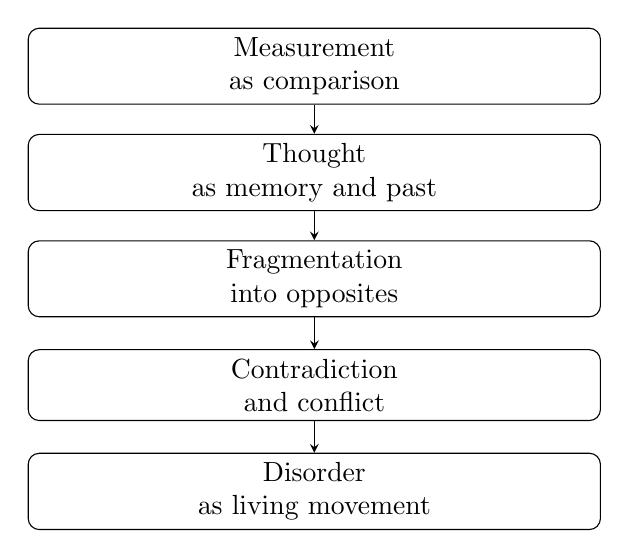
\begin{tikzpicture}[>=stealth]
\node[draw, rounded corners, align=center, text width=0.58\linewidth] (a) at (0,0) {Measurement\\as comparison};
\node[draw, rounded corners, align=center, text width=0.58\linewidth] (b) at (0,-1.35) {Thought\\as memory and past};
\node[draw, rounded corners, align=center, text width=0.58\linewidth] (c) at (0,-2.70) {Fragmentation\\into opposites};
\node[draw, rounded corners, align=center, text width=0.58\linewidth] (d) at (0,-4.05) {Contradiction\\and conflict};
\node[draw, rounded corners, align=center, text width=0.58\linewidth] (e) at (0,-5.40) {Disorder\\as living movement};
\draw[->] (a) -- (b);
\draw[->] (b) -- (c);
\draw[->] (c) -- (d);
\draw[->] (d) -- (e);
\end{tikzpicture}

A transcript-backed conceptual map of the lecture's middle movement. The arrows mark the order of inquiry, not a mechanical causal theory.
\end{figure}

\section{The Fact Without Comparison}

The lecture then tests whether one can look without measurement, that is, without comparison. Anderson's recollection of the dew on a lotus leaf gives the section its concrete force. At first he asks questions: where is the base, how can it be stable, why does it not roll off? Then the questioning exhausts itself, and he simply looks.

The story is not an ornament. It is a precise counterexample to comparison. The dew on the leaf is the fact. It does not have to be measured against something else in order to be seen. It is what is.

Krishnamurti takes the example into education. Can a student be educated to live without comparison? The ordinary educational structure compares from the beginning: clever and dull, successful and unsuccessful, better and worse. Krishnamurti reverses the premise. I know that I am dull only through comparison. If there is no comparison, I do not know myself through that label. Then I begin from there.

\begin{table}
\centering
\begin{tabular}{p{0.43\linewidth} p{0.43\linewidth}}
\textbf{Comparison} & \textbf{Non-comparative looking}\\
Measures one state against another & Begins with the fact as it is\\
Creates more and less & Does not move by hierarchy\\
Sustains anxiety and competition & Ends that particular conflict\\
Asks what I should become & Asks what is actually present\\
\end{tabular}

A compact contrast drawn from the conversation on measurement and comparison.
\end{table}

This is also where Anderson notices Krishnamurti's use of words like total and absolute. In context, those words do not mean dogmatic certainty. They mean that there is no bridge from total disorder to total order by gradual comparison. If the movement remains comparative, it remains inside measurement.

\section{Can The Disorderly Mind Observe Disorder?}

The most difficult question now appears. We have said that disorder must be understood. But the mind that is to understand disorder is itself disorderly. Can such a mind observe disorder?

\subsection{Question \& Answer}

\paragraph{Question.}
Can the mind, already in disorder, observe disorder without introducing an observer who imagines himself orderly?

\paragraph{Answer.}
Krishnamurti says that the imagined orderly observer is itself part of disorder. The observer who says, ``I am orderly, and I will put order into disorder,'' is the past. It is the maker of division. Therefore it is not outside the disorder it observes.

The central proposition is best written in the lecture's own plain form:

\begin{equation}
\text{observer}=\text{observed}.
\end{equation}

Later the same structure is stated as

\begin{equation}
\text{perceiver}=\text{perceived}.
\end{equation}

These are not algebraic identities. They are statements about division. The observer is memory, past, comparison, and fragmentation. When it stands apart from disorder as if it were clean, it has already divided the field. Where there is division, there is conflict; where there is conflict, there is disorder. Thus the observer cannot be the agent that brings order.

\begin{proposition}
A mind cannot bring order to disorder by inventing an observer separate from disorder.
\end{proposition}

\begin{proof}
The observer is introduced as an opposite to what is observed. But the observer is formed by thought, and thought is memory, past, and fragmentation. A fragment standing apart from another fragment produces division. Division produces conflict. Therefore the observer introduced as an ordering agent is itself a factor of disorder. It cannot bring order.
\end{proof}

The alternative is stated negatively: observe without the observer, perceive without the perceiver. This must not be converted into a technique. A technique requires a technician, a controller, a stiller of the mind; and that controller is another fragment of thought.

\begin{figure}
\centering
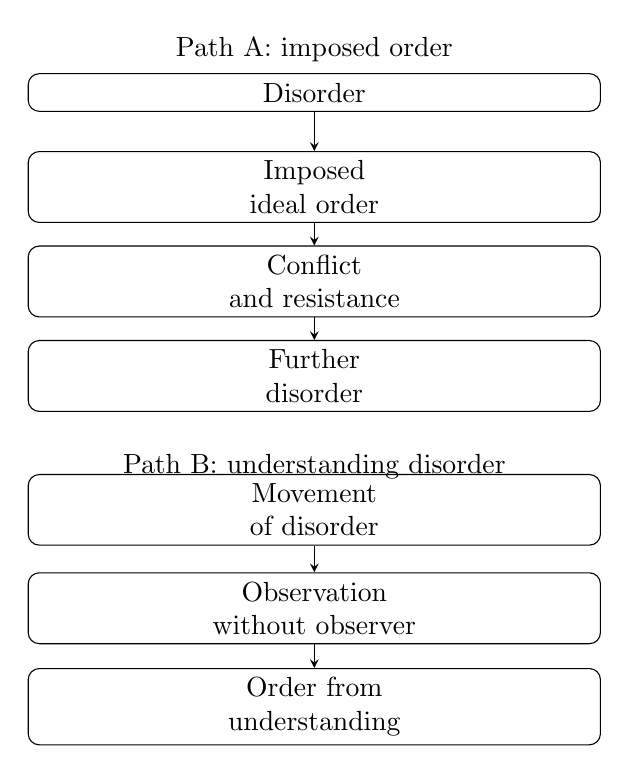
\begin{tikzpicture}[>=stealth]
\node[align=center] at (0,0.55) {Path A: imposed order};
\node[draw, rounded corners, align=center, text width=0.58\linewidth] (a1) at (0,0) {Disorder};
\node[draw, rounded corners, align=center, text width=0.58\linewidth] (a2) at (0,-1.20) {Imposed\\ideal order};
\node[draw, rounded corners, align=center, text width=0.58\linewidth] (a3) at (0,-2.40) {Conflict\\and resistance};
\node[draw, rounded corners, align=center, text width=0.58\linewidth] (a4) at (0,-3.60) {Further\\disorder};
\draw[->] (a1) -- (a2);
\draw[->] (a2) -- (a3);
\draw[->] (a3) -- (a4);

\node[align=center] at (0,-4.75) {Path B: understanding disorder};
\node[draw, rounded corners, align=center, text width=0.58\linewidth] (b1) at (0,-5.30) {Movement\\of disorder};
\node[draw, rounded corners, align=center, text width=0.58\linewidth] (b2) at (0,-6.55) {Observation\\without observer};
\node[draw, rounded corners, align=center, text width=0.58\linewidth] (b3) at (0,-7.80) {Order from\\understanding};
\draw[->] (b1) -- (b2);
\draw[->] (b2) -- (b3);
\end{tikzpicture}

A narrow transcript-backed contrast: superimposition continues disorder; observation without the observer is the lecture's proposed new factor.
\end{figure}

At this point Krishnamurti returns the disorder from ``out there'' to ``in here.'' War, national division, religious opposition, political corruption, and the search for separate solutions are not treated as external accidents. They are expressions of the same fragmented human mind. A divided mind tries to solve division by means of division, and the result is a series of palliatives.

\section{Order, Virtue, Conduct, And Attention}

After the observer discussion, Krishnamurti deliberately comes back to the central thesis: order comes only with the understanding of disorder. In that understanding there is no superimposition, no suppression, and no conflict. Order is now called a different kind of movement.

He then identifies that order with virtue. This must be read in light of the earlier warning about opposites. Virtue is not the opposite of vice. It is not an ideal projected against what is. Krishnamurti calls virtue conduct, and Anderson adds that the I Ching hexagram translated as conduct can also be translated as treading. The point is movement. Conduct is not a static moral pose; it is the movement of a life in order.

The final relation can be held as

\begin{equation}
\text{seeing the movement of disorder}
\longrightarrow
\text{order}
\longrightarrow
\text{virtue as conduct}.
\end{equation}

But if this line is made into a method, it has been misunderstood. The seeing is not produced by a controller. It is not a technique for stilling the mind. Anderson explicitly notices that a technique for stilling the mind requires a stiller, and that stiller is precisely the divided observer already exposed.

The lecture closes by returning to attention. Anderson begins to describe what happens when one thinks one is beginning to take the inquiry seriously, when one feels oneself leaning into it. At that point fear appears. The chapter therefore should not end as though the inquiry were complete. Order has been clarified, but the next door has opened: fear.

\section{Summary}

The conversation gives order both a negative and a positive precision. Negatively, order is not conformity, imitation, obedience, suppression, authority, or an ideal imposed upon disorder. Positively, order comes with the understanding of the movement of disorder.

That movement is traced through thought. Thought is the response of memory, experience, and the past; as such, it is fragmentary. Fragmentation becomes division, division becomes contradiction, and contradiction becomes conflict. Measurement, understood here as comparison, is one of the chief ways this movement continues in education, religion, hierarchy, self-image, and the desire to become.

The decisive statement is that the observer is the observed. The mind that tries to stand outside disorder and correct it is itself part of disorder, because it is made of the past and acts through division. Observation without the observer is therefore not a technique but a different quality of seeing. From that seeing, Krishnamurti says, order is not imposed. It flowers as virtue, conduct, responsibility, and attention, and it leads the inquiry directly toward fear.